\chapter{Sito in WordPress}
\label{chp:wp}
L'analisi dei requisiti ha evidenziato la necessità di un sito web in cui esporre e descrivere al cliente i servizi offerti, aggiornato e popolato da un componente del team di {\fem} senza per forza conoscenze e capacità tecniche informatiche; si è scelto quindi WordPress, un CMS molto diffuso.

{\wp} è una piattaforma software di content management system (CMS) ovvero un programma installato sul server che consente la creazione, gestione, distribuzione e manutenzione di un sito Internet \cite{wordpress}. è un progetto open-source creato da Matt Mullenweg e distribuito con la licenza GNU General Public License; è sviluppato in PHP con appoggio a MySQL come gestore di database.

{\wp} permette il download gratuito di tutti i suoi componenti dal sito \url{www.wordpress.org} per poterli installare sulla propria macchina. Esiste anche un servizio (a pagamento in base alle richieste) chiamato \emph{WordPress.com} che permette di costruire rapidamente il proprio sito web o blog basato su {\wp} senza la necessità di possedere un server o competenze tecniche specifiche.

\section{Caratteristiche di {\wp}}
{\wp} permette di estendere le proprie funzionalità con l'ausilio di opportuni plugin, ovvero moduli che aggiungono nuove caratteristiche ed elementi all'applicativo. I plugin possono essere gratuiti o a pagamento e possono fare molte fare di tutto, dal potenziare l'editor integrato di {\wp} all'inserire slideshow nelle pagine, e molto altro ancora. Come i plugin si possono trovare anche temi, estensioni che permettono di personalizzare l'aspetto del sito modificando sfondi, impaginazione, font, etc.

\section{{\wp} per avifauna.fem2ambiente.com}
Per realizzare il \emph{Portale della Diagnostica Molecolare dedicato all'Avifauna}, dopo aver scelto il sottodominio \texttt{www.avifauna.fem2ambiente.com}, si è prima di tutto installato e configurato {\wp}.

Per farlo è stato necessario scaricare l'ultima versione dal sito \url{www.wordpress.org} (ad oggi, Ottobre 2015, l'ultima versione è la 4.3.1) e seguire le istruzioni nel file \texttt{readme} \cite{installing_wordpress}, in particolare:
\begin{itemize}
\item eseguire le opportune modifiche al file \texttt{wp-config.php} in un editor di testo;
\item creare un database dedicato utilizzando MySQL;
\item connettersi al server e caricare tutti i file relativi l'installazione di {\wp} nella cartella scelta (\texttt{/home});
\item configurare in modo appropriato visitando la pagina 

\texttt{http://avifauna.fem2mabiente.com/home/wp-admin/install.php}
\end{itemize}

Una volta terminata l'installazione si è potuto procedere con l'installazione degli appropriati plugin, temi e estensioni.

La scelta del tema è ricaduta su \emph{Everest} di YOOtheme (Versione: 1.0.11). YOOtheme è una azienda tedesca che produce componenti per CMS \cite{yootheme}; i loro prodotti più importanti, oltre a una ventina di temi e template diversi rispettivamente per {\wp} e Joomla!, sono \emph{Wrap Framework} \cite{wrap} e \emph{Uikit} \cite{uikit}, due architetture software di supporto per la creazione e personalizzazione dei componenti aggiuntivi ai più famosi CMS.

Il tema Everest è stato costruito utilizzando Wrap Framework e mette a disposizione dell'utilizzatore sette stili di layout differenti, personalizzazioni nella costruzione del layout sfruttando tutte le potenzialità di {\wp} e un pacchetto di plugin chiamato \emph{Widgetkit} per l'inserimento rapido di Slideshow, gallierie di immagini, mappe. Per tutte queste caratteristiche è stato scelto, acquistato ed installato come tema per il sito.

Per ricoprire tutti i bisogni organizzativi di un sito commerciale come il Portale Avifauna è stato necessario installare anche plugin come \emph{Polylang} \cite{polylang} per il supporto multilingue al sito e \emph{My Calendar} \cite{mycalendar} per la gestione degli eventi.

Dopo aver creato popolato il sito con i contenuti, divisi in base alle pagine e sezioni dedicate, il risultato ottenuto è visibile nell'immagine~\ref{fig:homepage} e al seguente link \url{www.avifauna.fem2mabiente.com/home}.

\begin{figure}
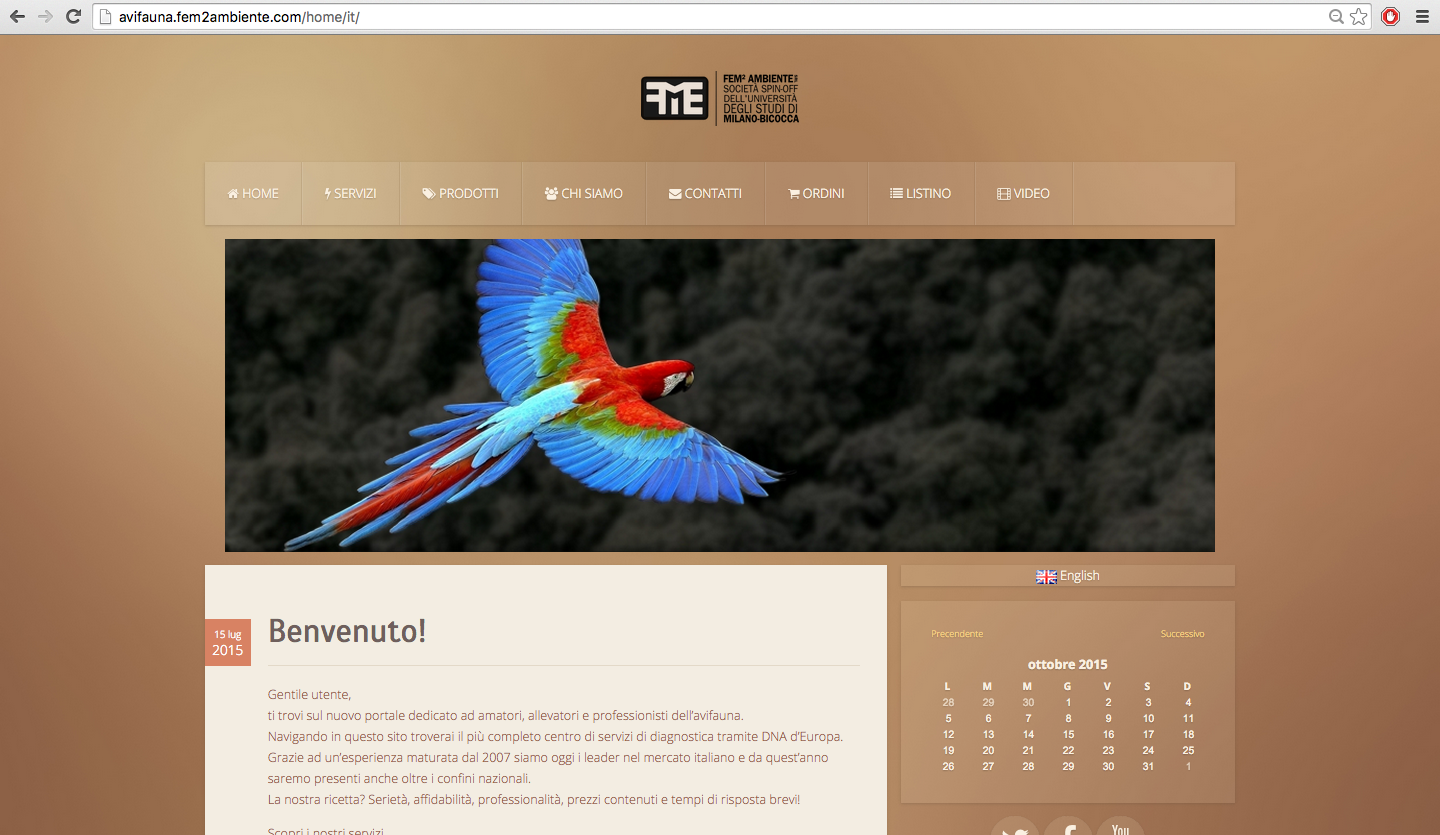
\includegraphics[width=1\textwidth]{images/homepage} 
\caption{homepage del Portale per la Diagnostica Molecolare Avifauna}
\label{fig:homepage}
\end{figure}

Cliccando sul tasto \textsf{Ordini} si può accedere alla piattaforma personalizzata, descritta nei seguenti capitoli.

\begin{center}
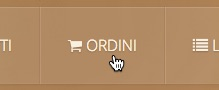
\includegraphics[width=0.3\textwidth]{images/homepage-ordini} 
\label{fig:homepage-ordini}
\end{center}